\documentclass[11pt]{article}
\usepackage{amsmath}
%\usepackage{extsizes}
\usepackage{amsmath,amssymb}
%\usepackage{omegavn,ocmrvn}
%\usepackage[utf8x]{inputenc}
\usepackage[utf8]{vietnam}

\usepackage{longtable}
\usepackage{answers}
\usepackage{graphicx}
\usepackage{array}
\usepackage{pifont}
\usepackage{picinpar}
\usepackage{enumerate}
\usepackage[top=3.0cm, bottom=3.5cm, left=3.5cm, right=2.5cm] {geometry}
\usepackage{hyperref}


\newtheorem{bt}{Câu}
\newcommand{\RR}{\mathbb R}
\Newassociation{sol}{Solution}{ans}
\newtheorem{ex}{Câu}
\renewcommand{\solutionstyle}[1]{\textbf{ #1}.}


\begin{document}
% \noindent
\begin{tabular*}
{\linewidth}{c>{\centering\hspace{0pt}} p{.7\textwidth}}
Trường ĐHKHTN, ĐHQGHN & {\bf Học Kỳ 1 (2018-2019)}
\tabularnewline
K61 TTƯD & {\bf Bài Tập Giải Tích Số. No 2}
\tabularnewline
\rule{1in}{1pt}  \small  & \rule{2in}{1pt} %(Due date:)
\tabularnewline

%  \tabularnewline
%  &(Đề thi có 1 trang)
\end{tabular*}
%
% \Opensolutionfile{ans}[ans1]

\begin{bt} 
a) Biết rằng $$\frac{\pi^4}{90}=1^{-4}+2^{-4}+3^{-4}+\dots.$$ Cần khoảng bao nhiêu số hạng để có thể tính $\frac{\pi^4}{90}$ với sai số tuyệt đối $0.5 \cdot 10^{-6}$.\\
b) Cần khoảng bao nhiêu số hạng trong khai triển Maclaurin để tính gần đúng $\cos(x)$ với $|x|<0.5$, chính xác đến 12 chữ số thập phân.
\end{bt}

\begin{bt}
a) Sử dụng thuật toán Horner đầy đủ để tìm các hệ số trong khai triển Taylor của hàm số sau tại $x=2$. 
%
\[
f(x)=3+7x-1.33 x^2 +19.2 x^4.
\]
%
b) Viết Matlab function dạng sau $y=Taylor(n,x0)$ trong đó $n$ là bậc của đa thức Taylor, $x0$ là điểm tại đó cần khai triển Taylor. Yêu cầu nhập vào các hệ số theo dạng vector/array $[a_0 \ a_1 ... \ a_n]$ và trả lại $y=[b_0 \ b_1 ... \ b_n]$. Test function đã viết cho hàm $f(x)$ trong câu a và $g(x)=\sin(x)$, $h(x)=\cos(x)$ tại $x0=0$.
\end{bt}

\begin{bt}
Sử dụng khai triển Taylor để biểu diễn $f(x+h)=\sin(\pi/4 + h)$ và tính gần đúng $sin(45.0005)$, làm tròn đến chín chữ số thập phân. 
Viết script để tính toán trong Matlab.
\end{bt}

\begin{bt}
Sử dụng những cách phù hợp để tránh sự "đánh mất một số chữ số chắc bởi phép trừ" trong các biểu thức sau
\begin{enumerate}
\item[i)] $f(x)=\sqrt{x+4}-2$ tại $x\approx 0$.
\item[ii)] $f(x)=1-sin(x)$ tại $x\approx \pi$.
\item[iii)] $f(x) = \cfrac{\sqrt{1+x^2}-1}{x^2} - \cfrac{x^2\sin x}{x-\tan x}$ tại $x\approx 0$.
\end{enumerate} 
\end{bt}

\begin{bt}
Tìm cách tính $f(x)=\cfrac{\cos x-e^{-x}}{\sin x}$ để tránh sự "đánh mất một số chữ số chắc bởi phép trừ" và hãy tính gần đúng $f(0.008)$ đến 10 chữ số thập phân.
\end{bt}

\begin{bt}
Viết công thức nghiệm của phương trình bậc hai $x^2-10^5x+1=0$. Viết script trên Matlab để tìm nghiệm và giải thích vì sao nếu sử dụng máy tính chỉ chính xác đến 8 chữ số thâp phân cho công thức nghiệm cổ điển thì có thể dẫn đến sự đánh mất một số chữ số chắc. Đưa ra giải pháp và kiểm tra sử dụng Matlab.
\end{bt}

\centerline{———————————Hết——————————-}

%\vspace{1cm}
%\noindent{\bf Chú ý:} {\it Cán bộ coi thi không giải thích gì thêm}\\
%\vspace{0.4cm}
%\noindent{\bf Họ và tên học sinh: \rule{3in}{.01pt} Lớp: \hrulefill}
%\Closesolutionfile{ans}
%\newpage
%\begin{center}
%{\LARGE{\bf ĐÁP ÁN}}
%\end{center}
%\begin{Solution}{1}
	\begin{figure}[h!]
		\centering
		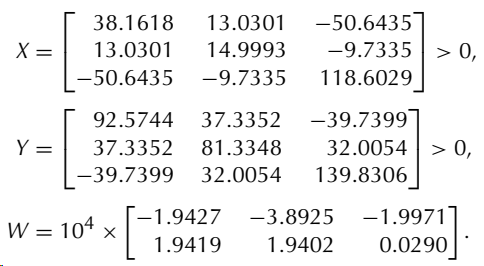
\includegraphics[width=0.7\linewidth]{Solution1/screenshot001}
		\caption[Exercise 1.2.5, Burden-Faires, 8ed.]{}
		\caption{}
		\label{fig:screenshot001}
	\end{figure}
\end{Solution}
 
   
\end{document}